\documentclass{article}

\usepackage{geometry}
\usepackage{amsmath}
\usepackage{graphicx}

\graphicspath{ {../results/} }
\geometry{
    a4paper,
    top=1in,
    left=1in
}

\title{Assignment-1 Report}
\author{S.Jaswanth-200050140, G.N.S.A.Siva Kishore-200050042}

\begin{document}
\maketitle
\newpage
$$ $$
\textbf{Report of question-1:}\\
    \\
    \textbf{Part-A/B}\\
    \\
    \textbf{Algorithm Explaination}:\\
    \textbf{Method of rejection:}\\
        Take that is valid from a data that already satisfies our prvious conditions.\\
    \textbf{Description:}\\
        Here we take a uniformly distributed points in a rectangle which is fairly simple
        and more over easy to generate. Thus we have the data which satisfies one of our 
        conditions which is the uniform spread. Now we just discard all the points which 
        are outside of our desired ellipse range which leaves a data set of uniformly spread
        points within an ellipse.\\
    \textbf{Downfall of algorithm:}\\
        If we are generating a fixed number of samples, say 100, points theoritically it may run forever and that is
        precisily because we are looping until we reach 100 succesful points. Nevertheless 
        practically it won't be the case because the random funtion numpy.random.uniform() is still
        a pseudo random number generator and there isn't any nartural randomness to only favour
        the luck to only get points outside the ellipse in the initial dataset generating the 
        uniform rectangle spread points.\\
    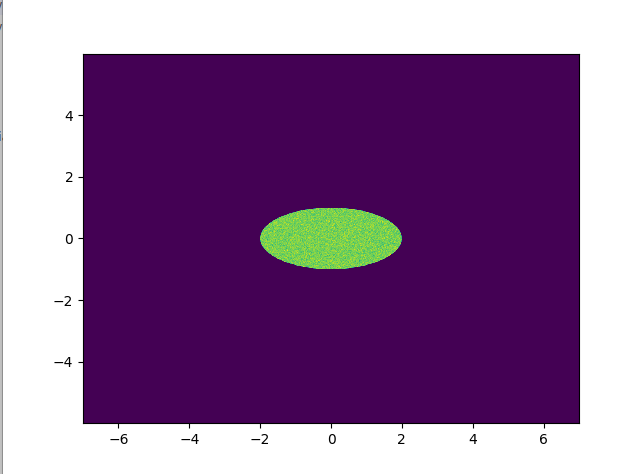
\includegraphics[scale=.6]{../results/q1/q1partA.png}\\
    \\
    \textbf{Part-C/D}\\
    \\
    \textbf{Algorithm Explaination:}\\
        Here we generate a point in a rectangle and according to it's one coordinate
        we shift the other coordinate so they all endup in our desired parallellogram and
        therefore in our desired triangle.\\
        It more like generating uniform points in a rectangle and modelling it's shape
        to match our parallelogram. And then divide the parallellogram in half to get uniform
        distribution in a desired triangle.\\
        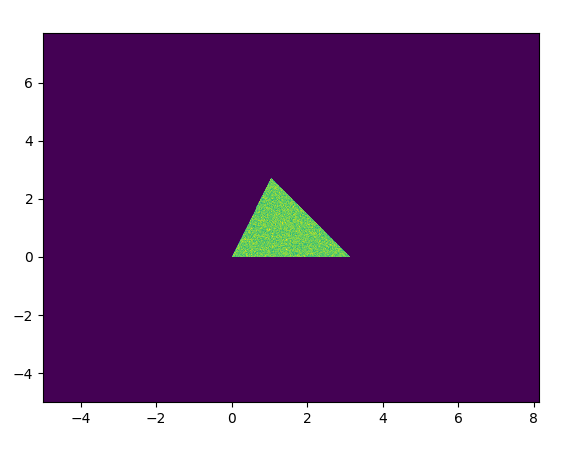
\includegraphics[scale=.6]{../results/q1/q1partC.png}\\
    \\
    \textbf{NOTE:}\\
    For detailed code and code walkthrough with comments please checkout the corresponding code file.\\

$$ $$
\textbf{Report of question-2:}\\
    \\
    \textbf{Algorithm:}\\
    General form of a multivariate matrix M would be\\
    $~~~~~~~~~~~~~~~~~~~~~~~~~~~~~~~~~$M = A*W + mean\\
    $~~~~~~~~~~$where W is a matrix formed by i.i.d independent standard gaussian ditributions.\\
    \\
    Let M' be M - mean\\
    $~~~~~~~~$M' = A*W
    \\
    Let M'=[m1,m2] and W=[w1,w1]\\
    \\
    $~~~~~~$From linear algebra we know that adding/subtracting one column from the other doesn't change
    it's eigen values nor eigen vectors so essentially we can obtain a lower triangular matrix for A
    and it works the same as the real/original A.\\

        If we are given a co-variance of a multivariate gaussian which is essentially the same as giving
    us the A which we require in order to convert two standard un-correlated gaussian distributions to their
    corresponding correlated multivariate distribution.\\

        This is because for a multi-variate gaussian of type "A*W + mean" covariance matrix is A*A`. From this
    we can obtain all the values assuming A to be a lower triangle and multiplying with it's transpose gives
    us n equations in n variables and we can find all these variables algebraically and obtain A.\\

        This is what is precisely done by the cholesky of linalg module of numpy. Or for our pupose we can define
    our own for a bi-variate as it's the most visuvalizable data in sense of plotting and representation.\\
    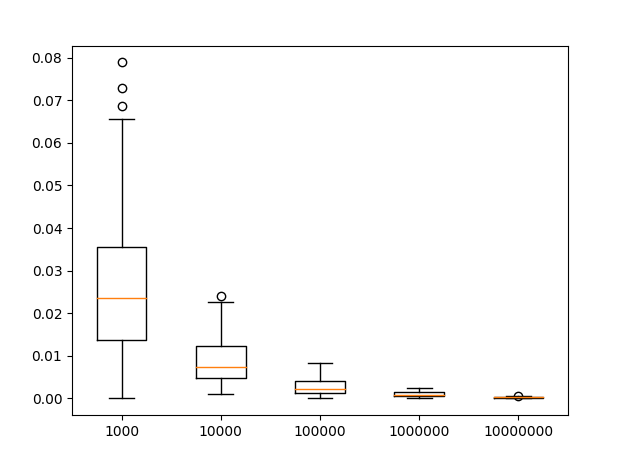
\includegraphics[scale=.6]{../results/q2/q2partB.png}\\
    The above is the resulting box plot over 100 iterations each in ML of mean. The exact same can be reproduced by running the
    corresponding pyhton code.\\
    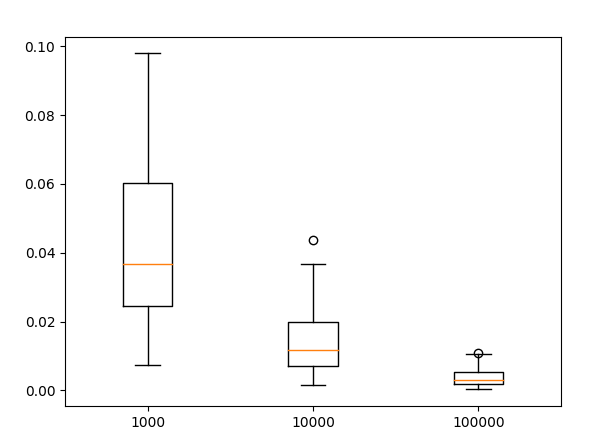
\includegraphics[scale=.6]{../results/q2/q2partC.png}\\
    The above is the resulting box plot over 100 iterations each in ML of norm of covariance. The exact same can be reproduced by running the
    corresponding pyhton code.\\
    \textbf{NOTE: My machine wasn't able to run 100 iterations each with a sample size of 10000000 for the covariance part. So I did only for upto 100000}
\newpage
$$ $$
\textbf{Report of question-3:}\\
    \\
    \textbf{Principle Component Analaysis:}\\
    $~~~~$This mainly focuses on reducing the dimentionality at the least expense of accuracy/loss of information\\
    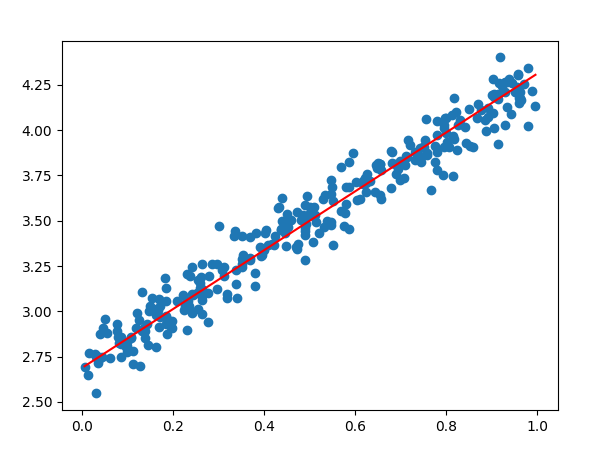
\includegraphics[scale=.5]{../results/q3/q3partB.png}\\
    Here from the scatter plot we can say that our original components X and Y are positive and lineaarly
    correlated and we can find a principle component from the eigen vectors of it's covariance which can give
    us the best approximation of linear relationship between the two original components because it captures
    most of the distributions spread and the spread perpendicular to this eigen vector direction is minimal
    which can be seen directly by the scatter plot or by analysing the corresponding eigen directions eigen value.\\
    $~~~~$We can implement an algorithm two ways, one is which involves the calculation covariance matrix and their 
    eigen vectors, other is by finding the line where the sum of squares of perpendicular distances from points to 
    that line which passes through mean will give the best approximate realtion between X and Y. Althought both results
    the same linear relation in X and Y.
    \\
    \\
    \textbf{Downfall of this linear PCA:} For a linear PCA approximation to work well the scattering should be nearly
    linear else the information loss will be big. This can be clearly seen when approximating a non-linear dataset.\\
    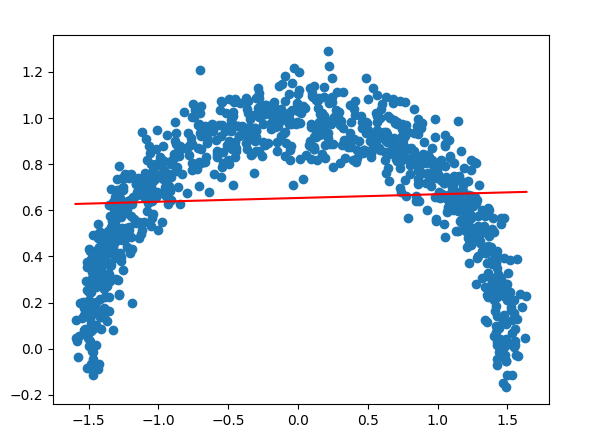
\includegraphics[scale=.6]{../results/q3/q3partC.png}\\
    The above is an example how our linear approximation deviates/loses too much information.
    \\
    \textbf{NOTE:}\\
    For the pure code implementation of above said algorithm please checkout the corresponding python code.

\newpage
$$ $$
\textbf{\large {Report of Question -4:}} \\
    \\
    \textbf{Part-A :} \\
         Mean can be caluculated by summating directly and then dividing it by number of repetetions for that digit.
    \\ \\
    \textbf{Part-B :} \\
        Covariance matrix is calucuted using the deviation vector.\\
        We will get covariance matrix when it deviation vector tranpose is multiplied by deviation vector.\\
         Deviation vector is nothing but vector having elements as standard deviation for each dimension \\ \\
    \textbf{Part- C :} \\
         The required values are caluculated by array manipulations.

    \textbf{Part - D :} \\
    $~~~~$ Considering the eigen values which are greater than the (largest eigen value/100),because there isn't much
    change wrt to the largest eigen value.
    \\
    $~~~~$ After executing the code the approximate principal modes obtained for each digit are :
    0-56,1-27,2-86,3-83,4-69,5-60,6-63,7-89,8-63,9-63.
    \\ \\
    $~~~~$ The Significant modes of variation are far less when compared to 784. \\
    Consider a specific digit for example 1 here almost the principal modes are only in specific pixels than 
    covering the enitre range of the image(28x28).Due to this we can almost assume that if we write it in a different way, the pixels
    adjacent to it are affected but not all. So for a specific digits we will have different modes of variation.
    \\ \\ \\
    \textbf{Eigen value Plots :} \\ \\
    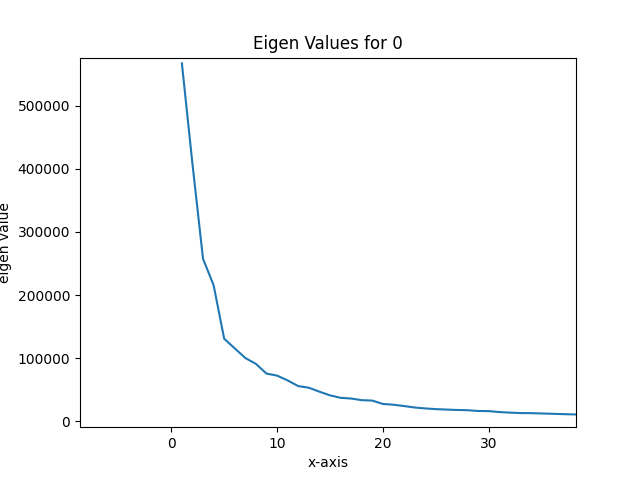
\includegraphics[scale=.5]{../results/q4/eigen_plots/0_eigen_value.png}
    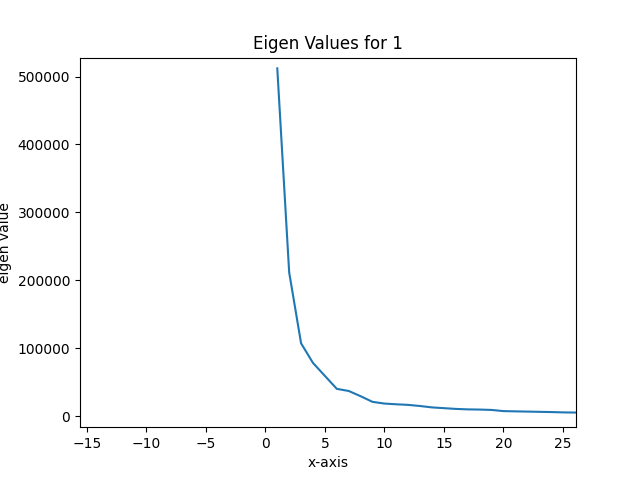
\includegraphics[scale=.5]{../results/q4/eigen_plots/1_eigen_value.png}
    \\
    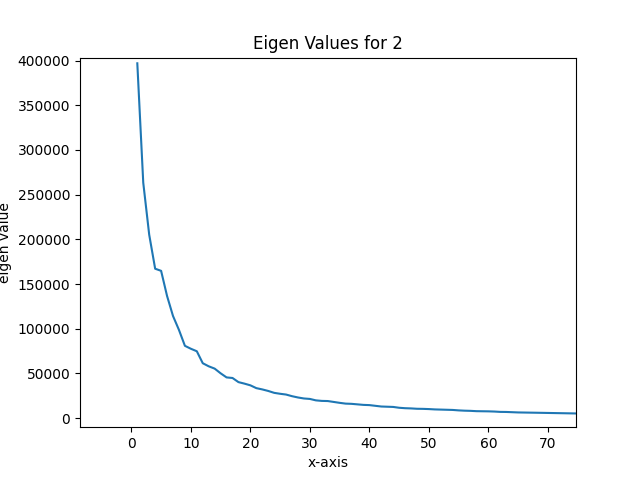
\includegraphics[scale=.5]{../results/q4/eigen_plots/2_eigen_value.png}
    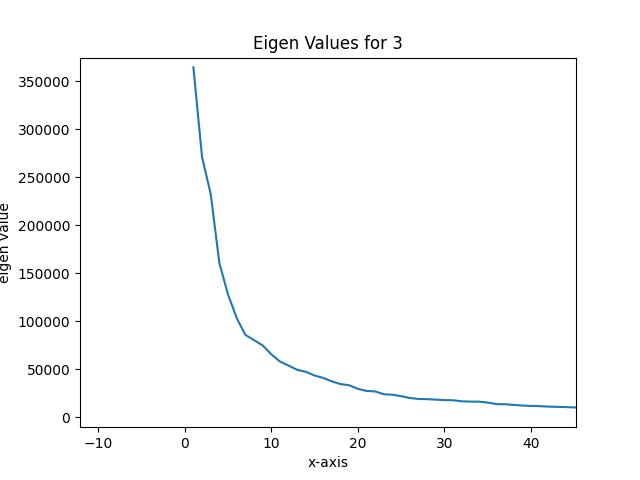
\includegraphics[scale=.5]{../results/q4/eigen_plots/3_eigen_value.png}
    \\
    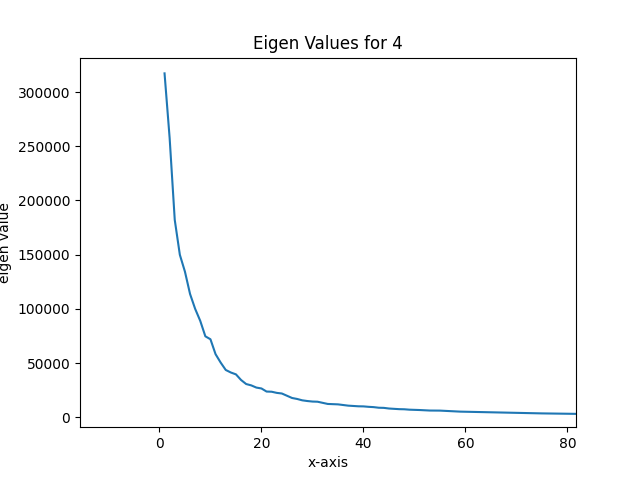
\includegraphics[scale=.5]{../results/q4/eigen_plots/4_eigen_value.png}
    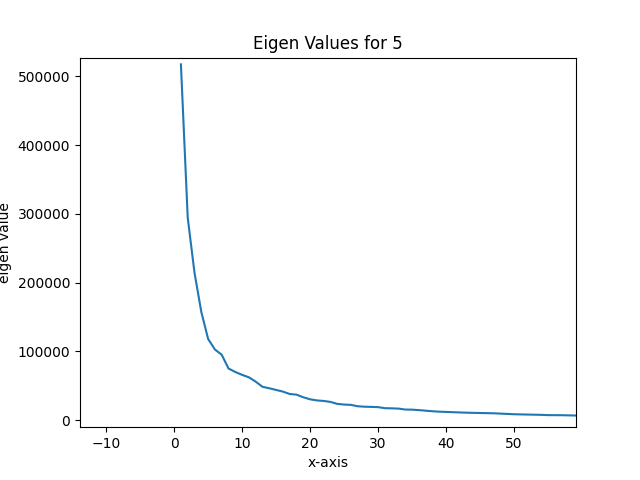
\includegraphics[scale=.5]{../results/q4/eigen_plots/5_eigen_value.png}
    \\
    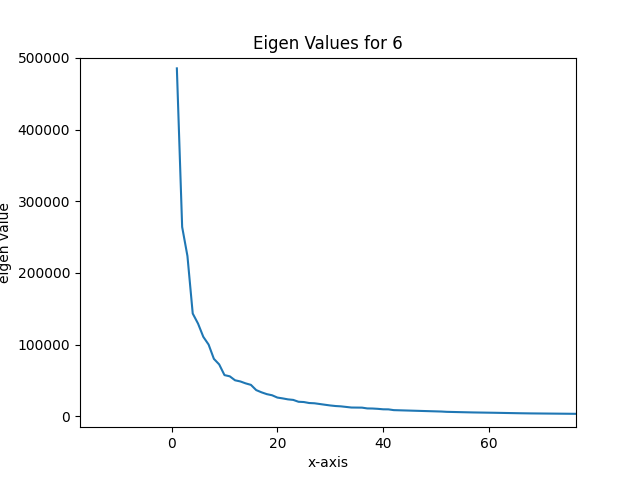
\includegraphics[scale=.5]{../results/q4/eigen_plots/6_eigen_value.png}
    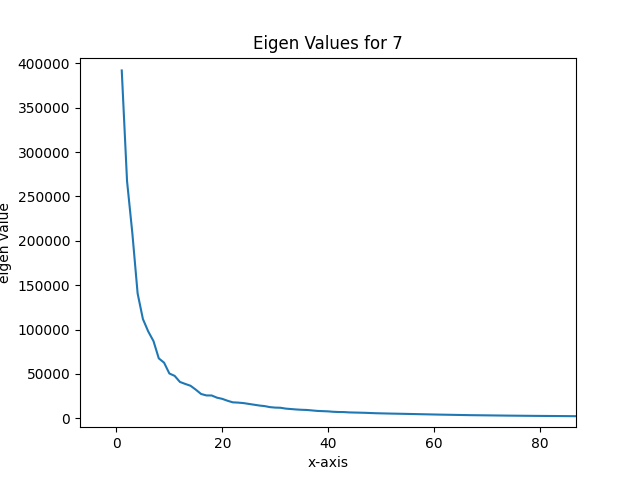
\includegraphics[scale=.5]{../results/q4/eigen_plots/7_eigen_value.png}
    \\
    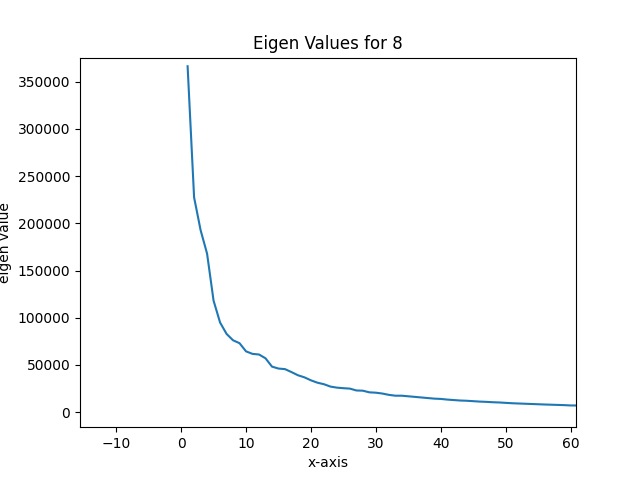
\includegraphics[scale=.5]{../results/q4/eigen_plots/8_eigen_value.png}
    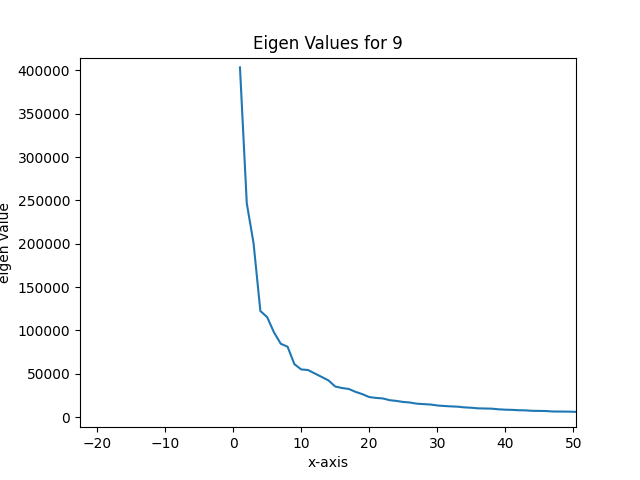
\includegraphics[scale=.5]{../results/q4/eigen_plots/9_eigen_value.png}
    \\ \\ \\
    \textbf{Part - E :} \\ \\
    $~~~~$ Let's take the graph for digit 1 when we subtract the given component along the principal mode direction,
    We know that along the principal significant mode the values in the pixels vary diversified.So the image we will be getting is almost a dull 
    intensity reduced image.
    \\ \\ 
    $~~~~$Where as in case of adding the component the other pixels dont get changed where as the pixels in which
    , the digit is present gets slightly intensified. 
    \\ \\
    $~~~~$ Clearly we can see when we subtracted the given principal components almost all we can see a whitish image,
    which implies the way people write the digit 1 is such that it's variance is maximized in that direction.
    \\ \\ \\

    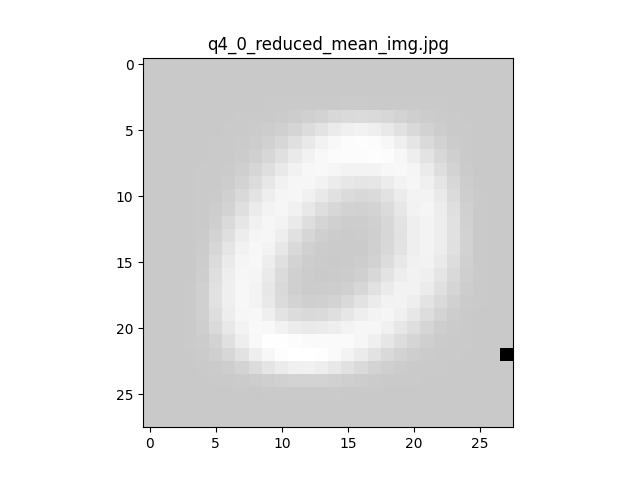
\includegraphics[scale=.37]{../results/q4/reduced_mean_images/q4_0_reduced_mean_img.png}
    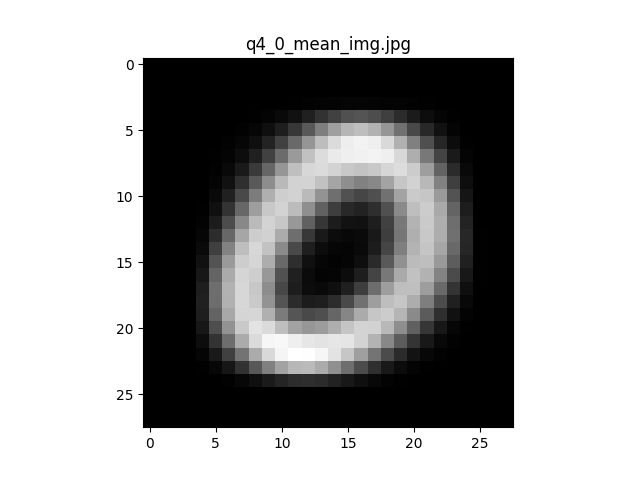
\includegraphics[scale=.37]{../results/q4/mean_images/q4_0_mean_img.png}
    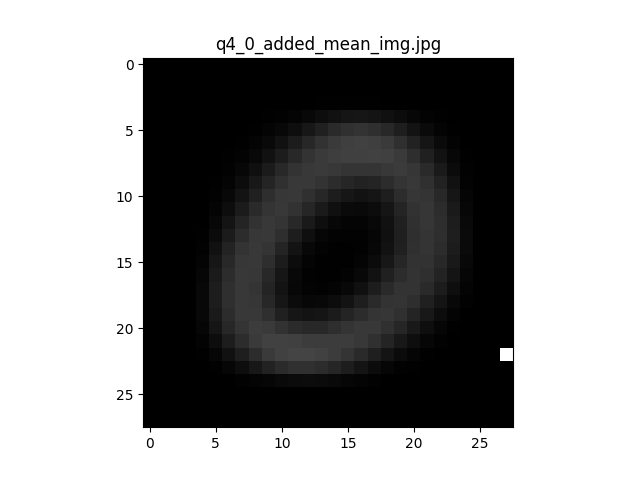
\includegraphics[scale=.37]{../results/q4/added_mean_images/q4_0_added_mean_img.png}
    \\
    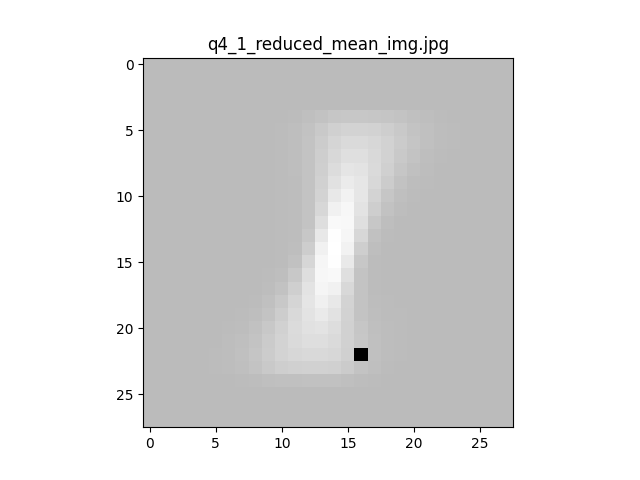
\includegraphics[scale=.37]{../results/q4/reduced_mean_images/q4_1_reduced_mean_img.png}
    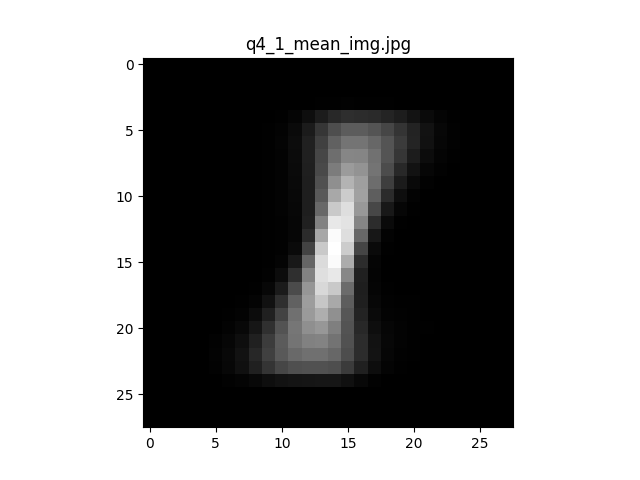
\includegraphics[scale=.37]{../results/q4/mean_images/q4_1_mean_img.png}
    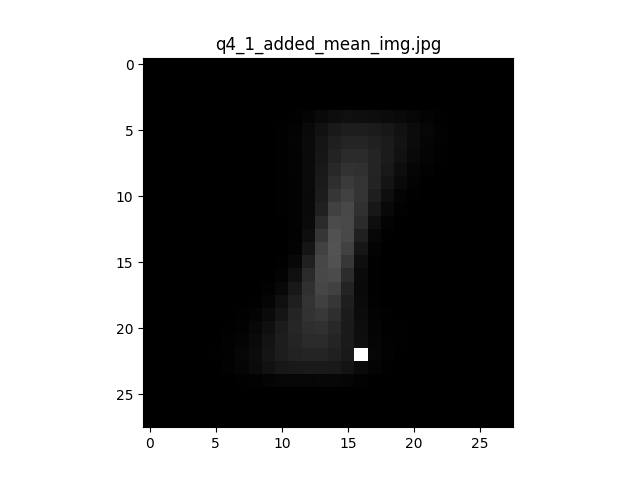
\includegraphics[scale=.37]{../results/q4/added_mean_images/q4_1_added_mean_img.png}
    \\
    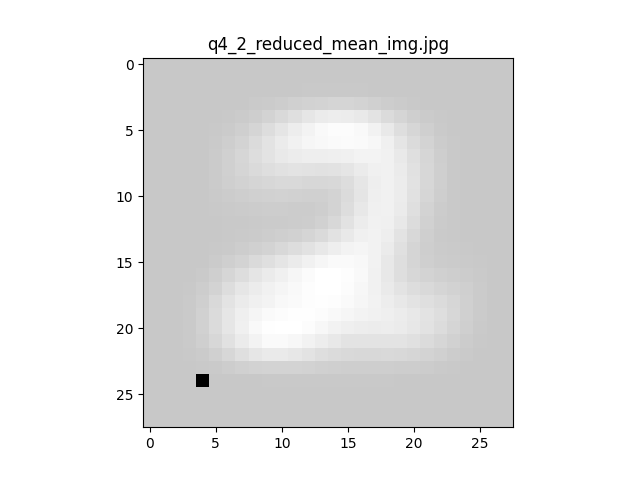
\includegraphics[scale=.37]{../results/q4/reduced_mean_images/q4_2_reduced_mean_img.png}
    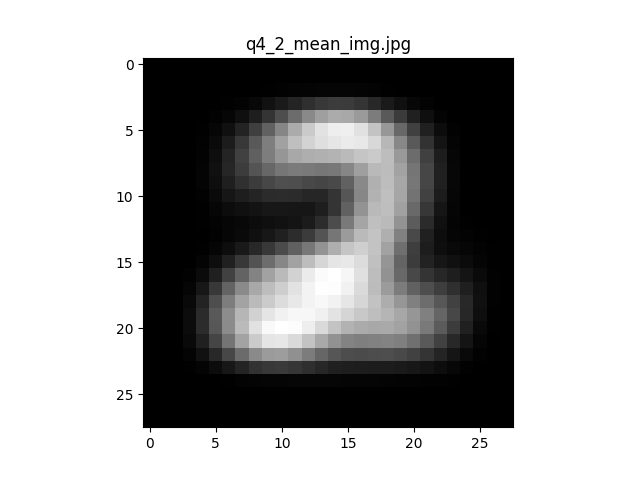
\includegraphics[scale=.37]{../results/q4/mean_images/q4_2_mean_img.png}
    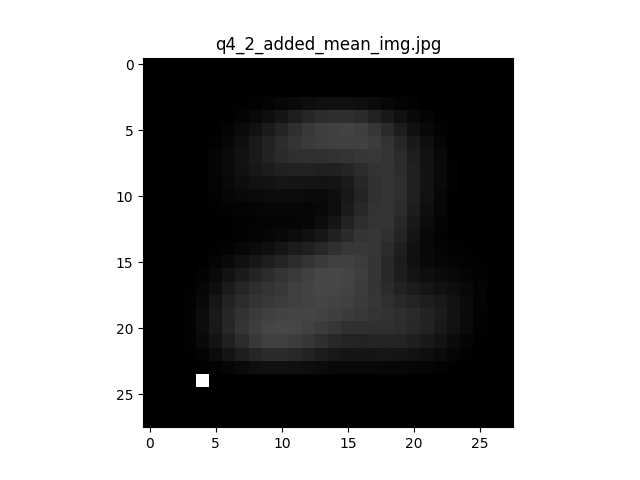
\includegraphics[scale=.37]{../results/q4/added_mean_images/q4_2_added_mean_img.png}
    \\
    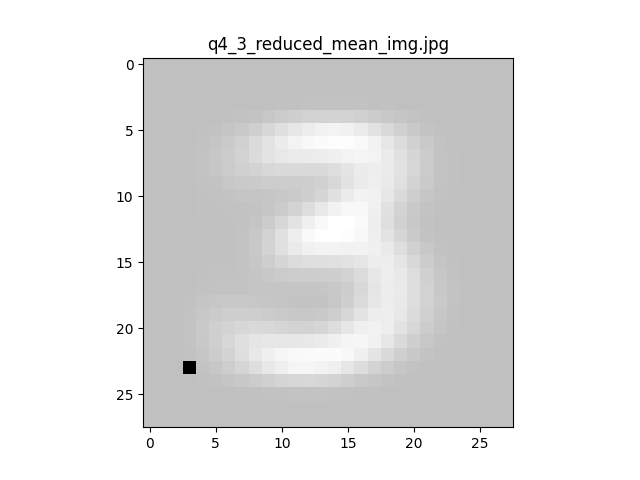
\includegraphics[scale=.37]{../results/q4/reduced_mean_images/q4_3_reduced_mean_img.png}
    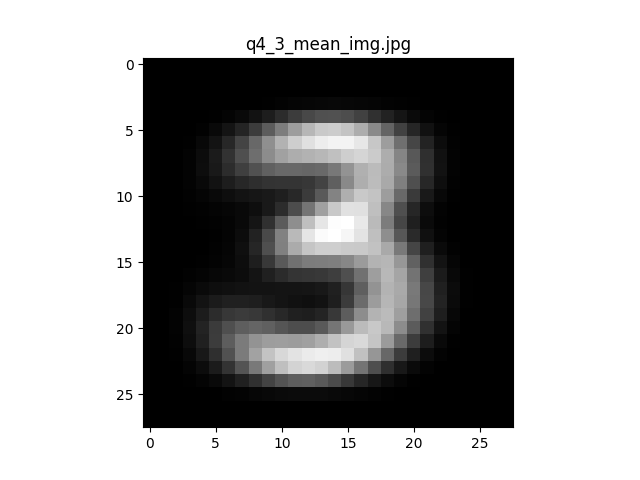
\includegraphics[scale=.37]{../results/q4/mean_images/q4_3_mean_img.png}
    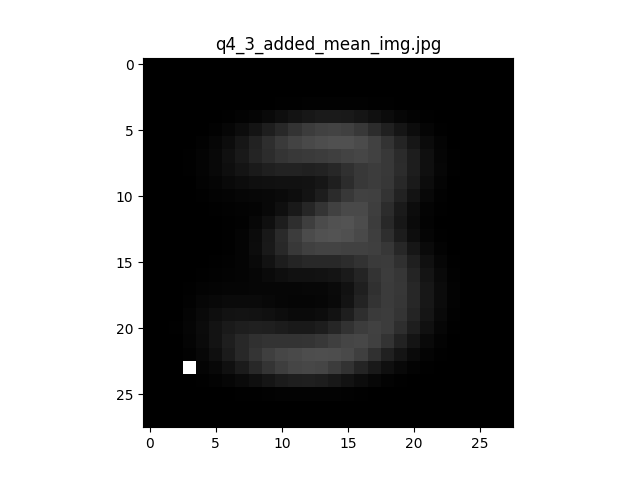
\includegraphics[scale=.37]{../results/q4/added_mean_images/q4_3_added_mean_img.png}
    \\
    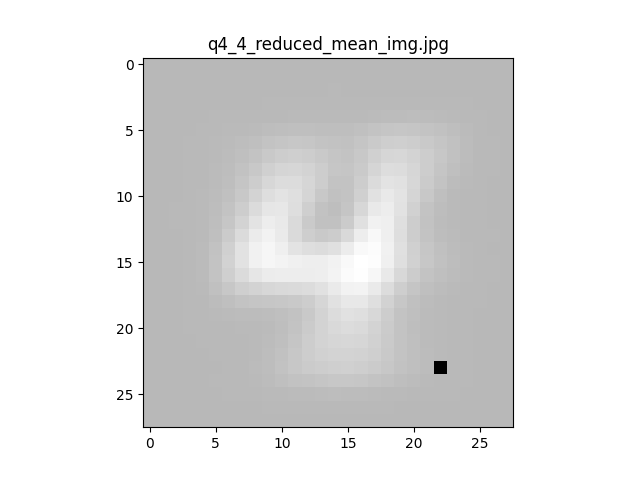
\includegraphics[scale=.37]{../results/q4/reduced_mean_images/q4_4_reduced_mean_img.png}
    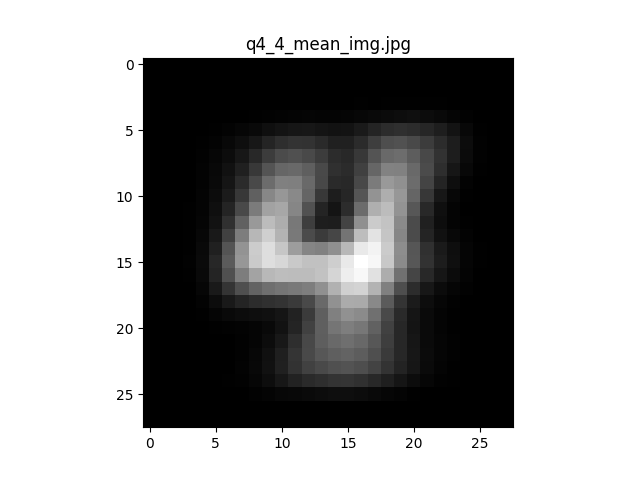
\includegraphics[scale=.37]{../results/q4/mean_images/q4_4_mean_img.png}
    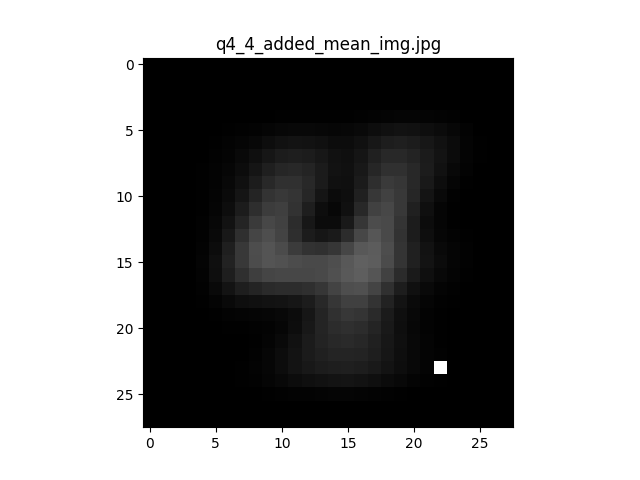
\includegraphics[scale=.37]{../results/q4/added_mean_images/q4_4_added_mean_img.png}
    \\
    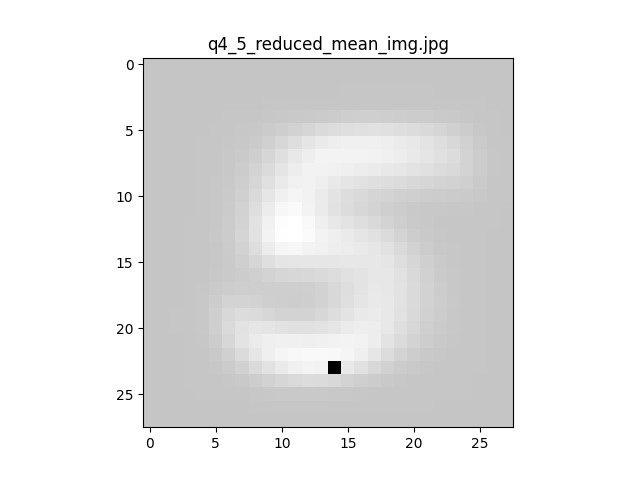
\includegraphics[scale=.37]{../results/q4/reduced_mean_images/q4_5_reduced_mean_img.png}
    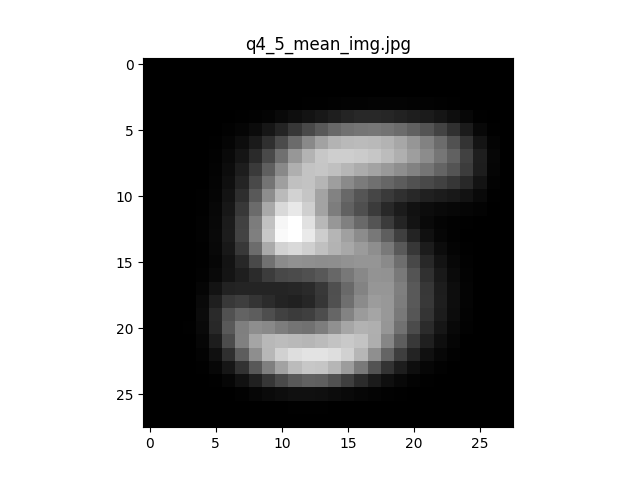
\includegraphics[scale=.37]{../results/q4/mean_images/q4_5_mean_img.png}
    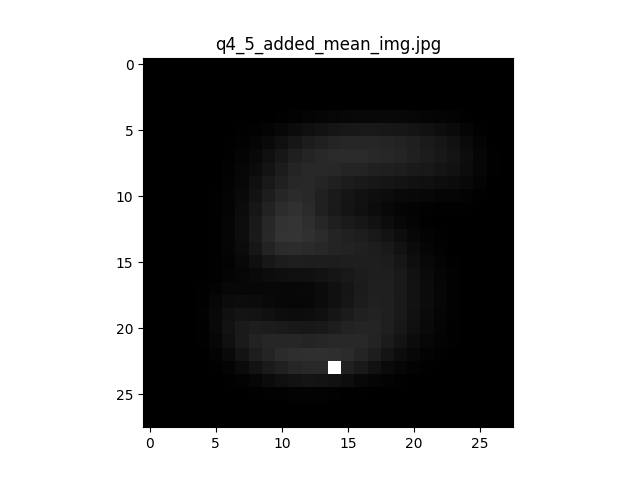
\includegraphics[scale=.37]{../results/q4/added_mean_images/q4_5_added_mean_img.png}
    \\
    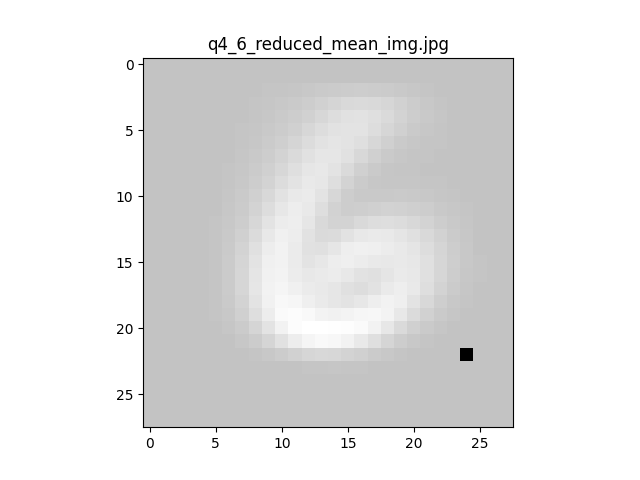
\includegraphics[scale=.37]{../results/q4/reduced_mean_images/q4_6_reduced_mean_img.png}
    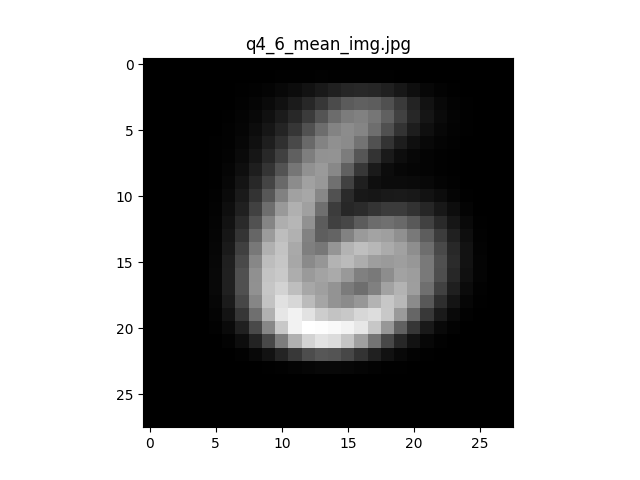
\includegraphics[scale=.37]{../results/q4/mean_images/q4_6_mean_img.png}
    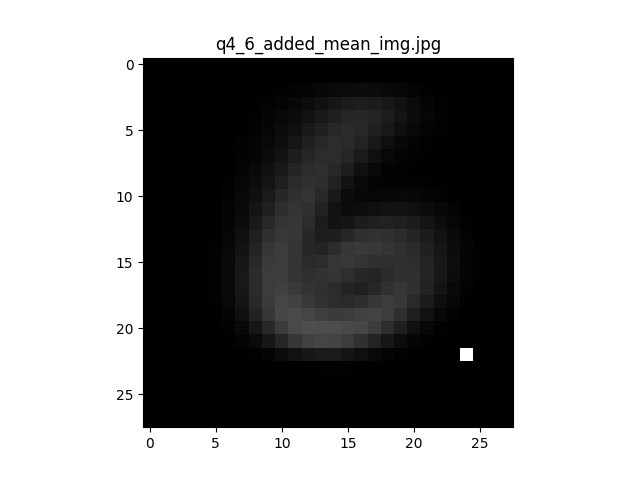
\includegraphics[scale=.37]{../results/q4/added_mean_images/q4_6_added_mean_img.png}
    \\
    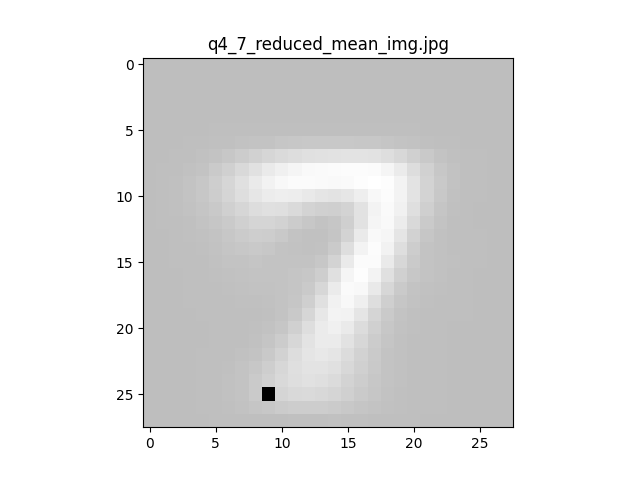
\includegraphics[scale=.37]{../results/q4/reduced_mean_images/q4_7_reduced_mean_img.png}
    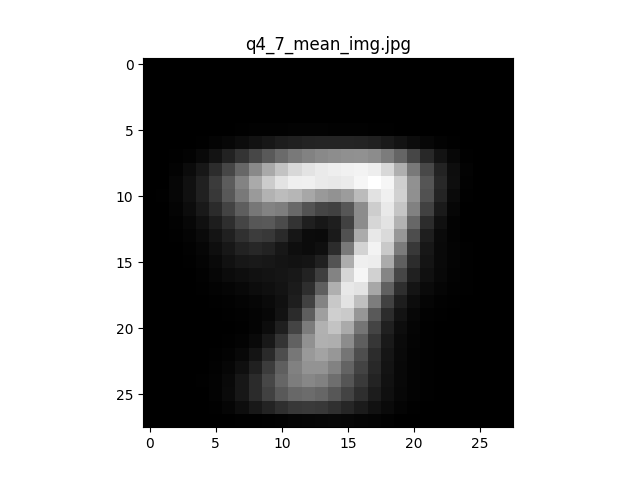
\includegraphics[scale=.37]{../results/q4/mean_images/q4_7_mean_img.png}
    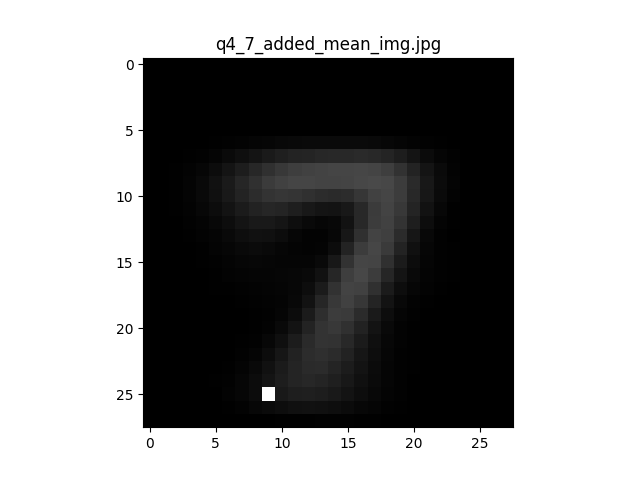
\includegraphics[scale=.37]{../results/q4/added_mean_images/q4_7_added_mean_img.png}
    \\
    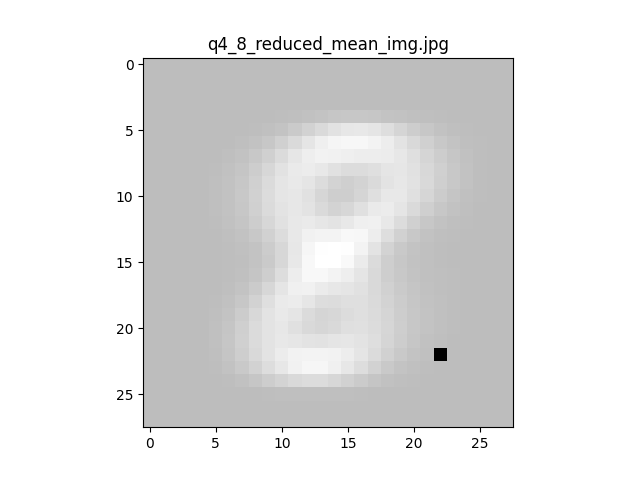
\includegraphics[scale=.37]{../results/q4/reduced_mean_images/q4_8_reduced_mean_img.png}
    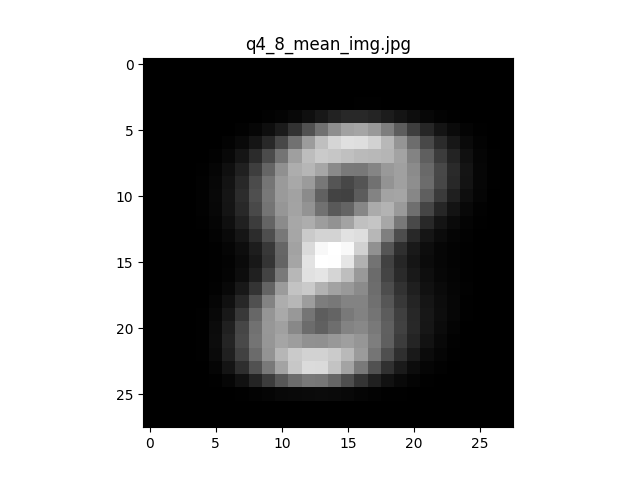
\includegraphics[scale=.37]{../results/q4/mean_images/q4_8_mean_img.png}
    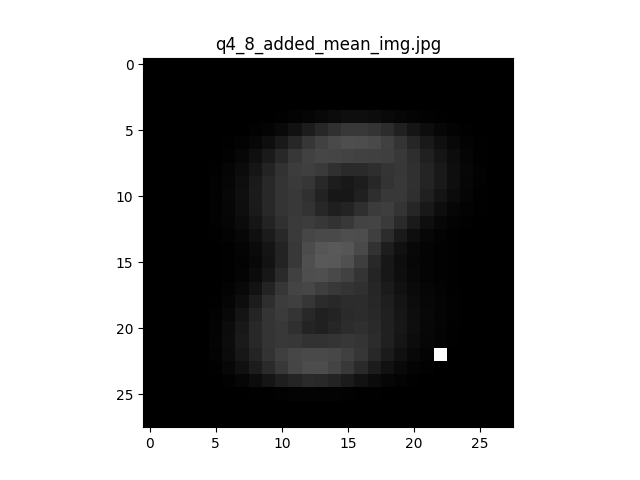
\includegraphics[scale=.37]{../results/q4/added_mean_images/q4_8_added_mean_img.png}
    \\
    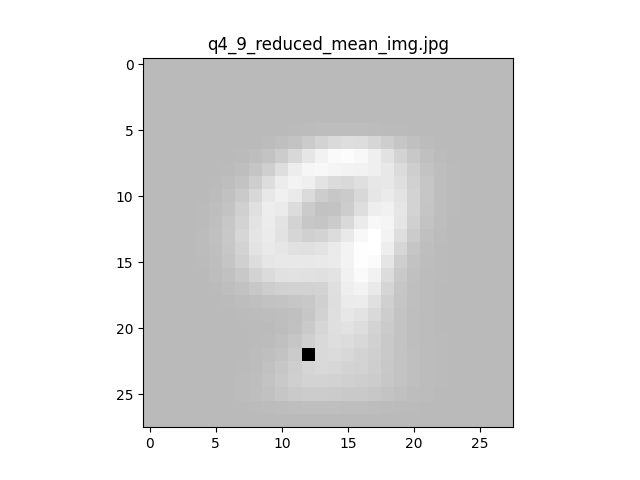
\includegraphics[scale=.37]{../results/q4/reduced_mean_images/q4_9_reduced_mean_img.png}
    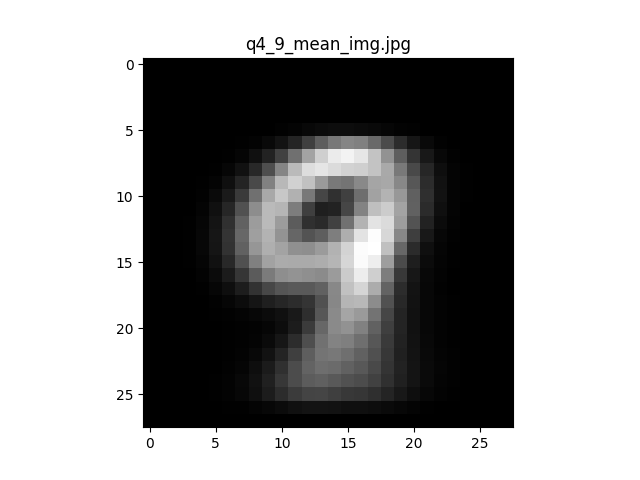
\includegraphics[scale=.37]{../results/q4/mean_images/q4_9_mean_img.png}
    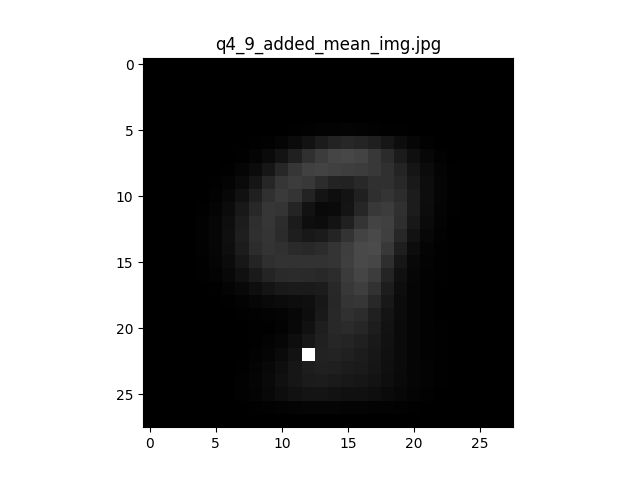
\includegraphics[scale=.37]{../results/q4/added_mean_images/q4_9_added_mean_img.png}


$$ $$ 
\textbf{\large {Report of Question -5:}} \\ \\
    \textbf{Part - A :} \\
    $~~~~$The PCA function written in the code will return list of the 84 co-ordinates caluculated.
    \\ \\ 
    \textbf{Part-B :} \\
    $~~~~$ We can construct the 84 co-ordinates by using the first 84 eigen vectors in the sorted list of total eigen vectors,
    and for constructing the image using these 84 coordinates we again do some matrix manipulations using the same 84 eigen vectors,
    to get the final 28x28 values. \\ \\
    \textbf{NOTE:}\\
    For the pure code implementation of above said algorithm please checkout the corresponding python code.
    \\ \\
    \newpage
    \textbf{\large Comparision between the Original and Reconstructed Images :} \\
    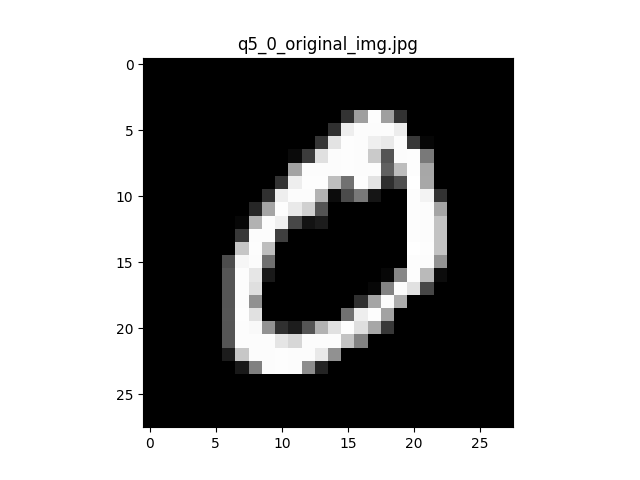
\includegraphics[scale=.6]{../results/q5/original/q5_0_original.png}
    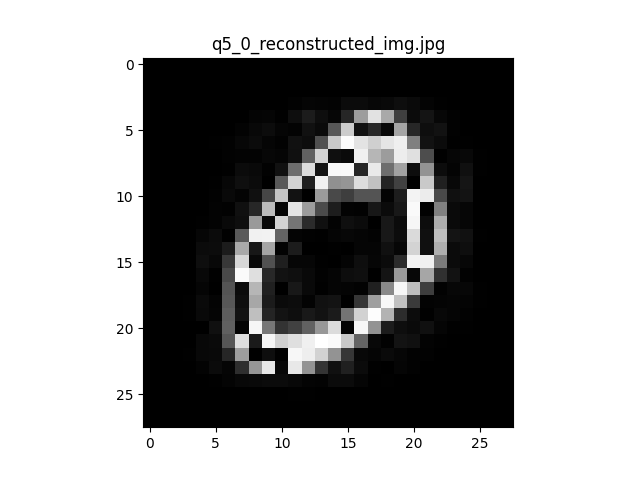
\includegraphics[scale=.6]{../results/q5/reconstrcuted/q5_0_reconstructed.png}
    \\
    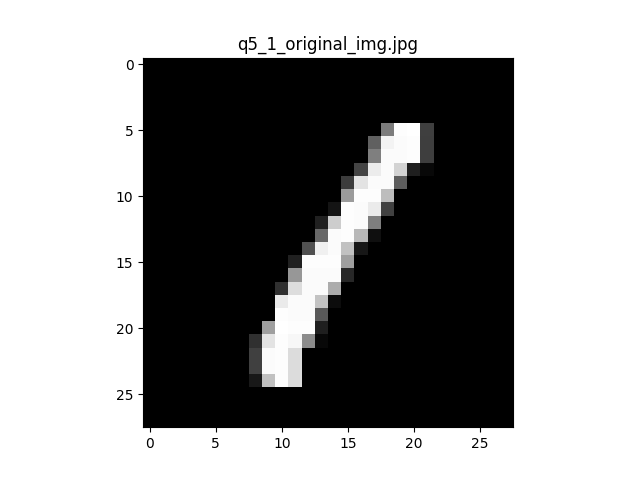
\includegraphics[scale=.6]{../results/q5/original/q5_1_original.png}
    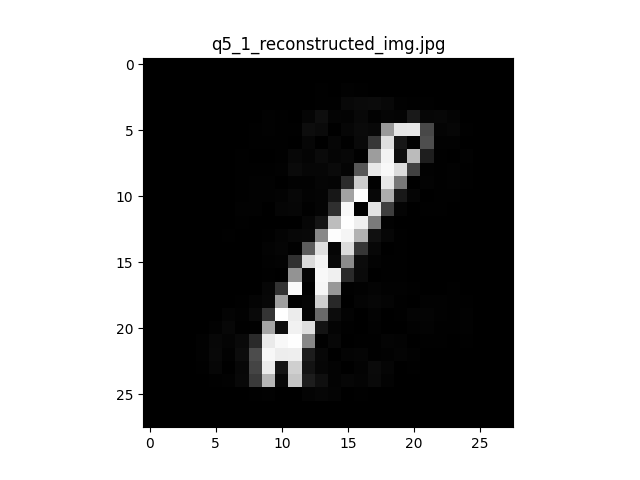
\includegraphics[scale=.6]{../results/q5/reconstrcuted/q5_1_reconstructed.png}
    \\
    \includegraphics[scale=.6]{../results/q5/original/q5_2_original.png}
    \includegraphics[scale=.6]{../results/q5/reconstrcuted/q5_2_reconstructed.png}
    \\
    \includegraphics[scale=.6]{../results/q5/original/q5_3_original.png}
    \includegraphics[scale=.6]{../results/q5/reconstrcuted/q5_3_reconstructed.png}
    \\
    \includegraphics[scale=.6]{../results/q5/original/q5_4_original.png}
    \includegraphics[scale=.6]{../results/q5/reconstrcuted/q5_4_reconstructed.png}
    \\
    \includegraphics[scale=.6]{../results/q5/original/q5_5_original.png}
    \includegraphics[scale=.6]{../results/q5/reconstrcuted/q5_5_reconstructed.png}
    \\
    \includegraphics[scale=.6]{../results/q5/original/q5_6_original.png}
    \includegraphics[scale=.6]{../results/q5/reconstrcuted/q5_6_reconstructed.png}
    \\
    \includegraphics[scale=.6]{../results/q5/original/q5_7_original.png}
    \includegraphics[scale=.6]{../results/q5/reconstrcuted/q5_7_reconstructed.png}
    \\
    \includegraphics[scale=.6]{../results/q5/original/q5_8_original.png}
    \includegraphics[scale=.6]{../results/q5/reconstrcuted/q5_8_reconstructed.png}
    \\
    \includegraphics[scale=.6]{../results/q5/original/q5_9_original.png}
    \includegraphics[scale=.6]{../results/q5/reconstrcuted/q5_9_reconstructed.png}

$$ $$  
\textbf{\large Report of Question-6 :} \\
\textbf{Part - A :} \\
    $~~~~$ Mean is caluculated as in the same way we did in the question 4.
    Same for the covariance matrix also but here we will be getting a 19200x19200 matrix.
    For which caluculation of eigen values and eigen vectors is taking a lot of runtime.
    \\
    $~~~~$ To obtain the eigen values we have used function eigh() from np.linalg.
    For obtaining deviation vector we have used function stdev() from statistics.
    \\ \\
    \textbf{\large mean image :} \\
    \includegraphics[scale = .6]{q6/mean_image.png}\\
    \\ \\
    Due to time factor (CS251 project presentation,CS213 quiz )we were not able to do the question completly and when we run the code,
    it is taking more than 20 minutes each time, so we were not able to complete this question.



\end{document}